\section{VSWR vs Frequency}

A good way to tell if an antenna is well-matched at a given frequency is to
calculate its Voltage Standing Wave Ratio. This can be calculated by
Equation(\ref{eq:vswr}):
\begin{align}
  \text{VSWR}&=\bigg(\frac{1+|\Gamma|}{1-|\Gamma|}\bigg)\quad
  \text{VSWR}\in(1,\infty)\label{eq:vswr}
\end{align}
\begin{align*}
  \Gamma&=\bigg(\frac{V_{Reflected}}{V_{Incoming}}\bigg)=\bigg(\frac{Z_A-Z_0}{Z_A+Z_0}\bigg)\quad\Gamma\in(0,1)
\end{align*}
Given that our reference impedance $Z_0$ was $50 \Omega$, our VSWR was found to
be 1.433 at 7MHz. This can be observed as the minimum in the plot of VSWR
against frequency shown in Figure~\ref{fig:vswr}.

\begin{figure}[h!]
  \centering
  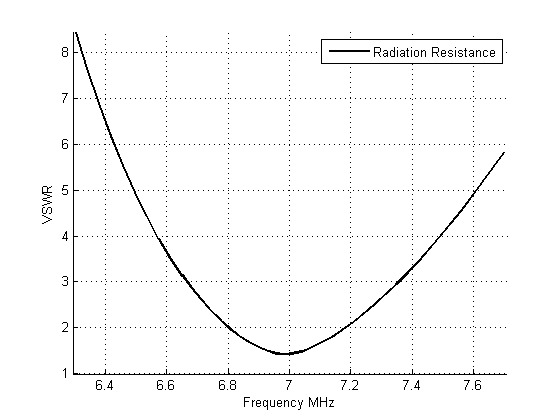
\includegraphics[width=0.45\textwidth]{./img/vswr.png}
  \caption{VSWR versus frequency}
  \label{fig:vswr}
\end{figure}

